Data for glider:


$C_D = 0.01 + 0.022C_l^2, \quad m = 454_{kg}, \quad S = 7.43_{m^2}$


$\to C_{D_0} = 0.01, \quad K = 0.022$


Glider is in $(\dfrac{L}{D})_{\max}$

$(\dfrac{L}{D})_{\max} = \dfrac{1}{\sqrt{4C_{D_0}K}} = \dfrac{1}{\sqrt{4\times 0.01 \times 0.022}} = 33.7100$


In $(\dfrac{L}{D})_{\max}$:


$\dfrac{1}{(L/D)_{\max}} = \dfrac{C_{D_0}}{C_l} + K C_l = \dfrac{1}{33.71} = \dfrac{0.01}{C_l} + 0.022 C_l $ 


Above equation Solved in MATLAB and code(Q3.m) attached.


From MATLAB solution:
$$C_l = 0.674\to C_D = 0.02$$ 
Assume:


$\gamma = -\tan^{-1}(\dfrac{1}{(L/D)_{\max}}) \to \gamma = -0.0297_{rad}$


For equilibrium condition $\dot{\gamma} = 0 
\to \dfrac12 C_l  \rho V^2S/m = g\cos(\gamma)$
$$\to V_{eq} = \sqrt{\dfrac{2mg\cos(\gamma_{eq})}{C_l \rho S}}$$
In MATLAB code we use ISA to plot $V_{eq}$ for altitude 0 to 5000 ft.
$\gamma_{eq}$ is constant in every altitude.
$$\gamma_{eq} = -0.0297_{rad}$$
\begin{figure}[H]
	\caption{$V_{eq} in different altitude$}
	\centering
	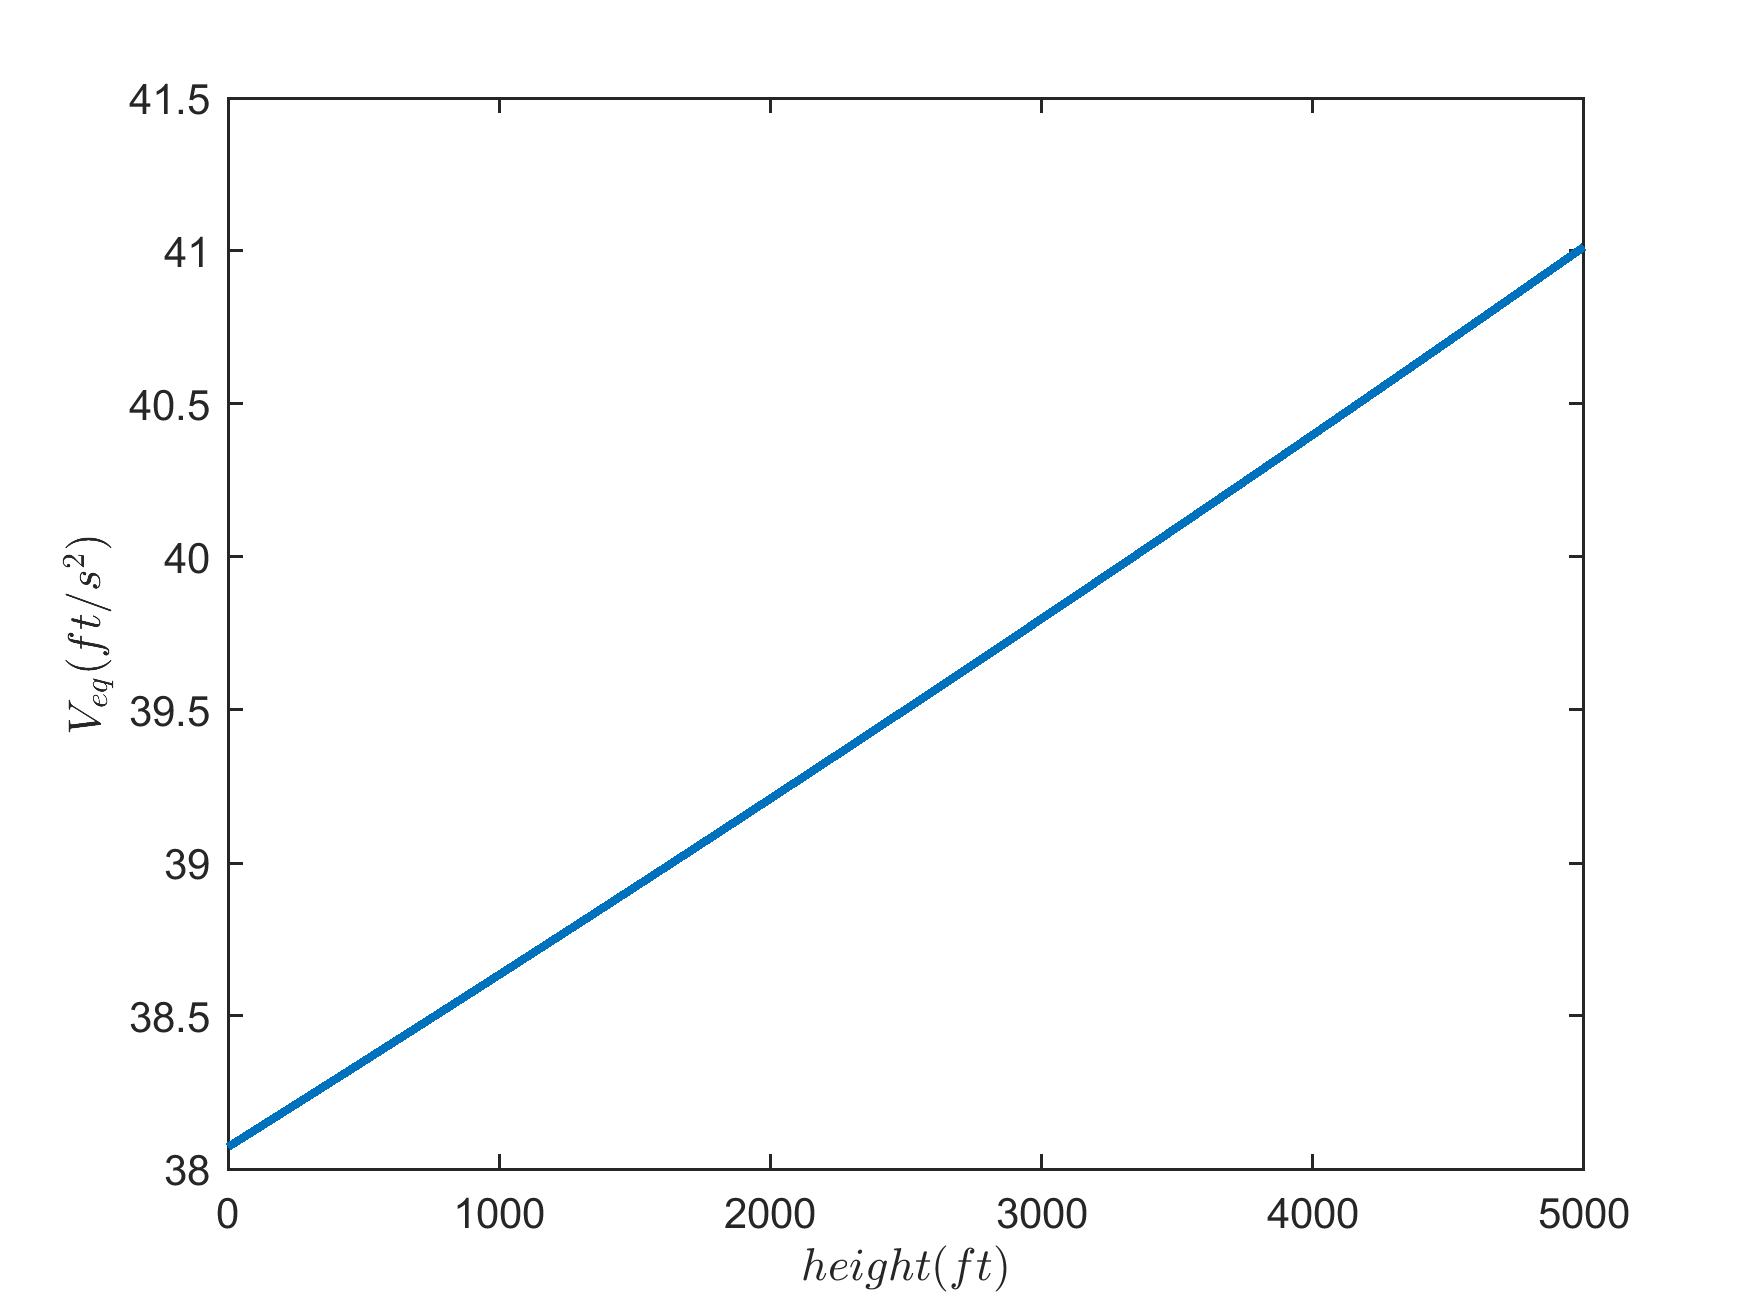
\includegraphics[width=12cm]{Q3/figures/V_eq.png}
\end{figure}
